% Options for packages loaded elsewhere
\PassOptionsToPackage{unicode}{hyperref}
\PassOptionsToPackage{hyphens}{url}
%
\documentclass[
]{book}
\usepackage{lmodern}
\usepackage{amssymb,amsmath}
\usepackage{ifxetex,ifluatex}
\ifnum 0\ifxetex 1\fi\ifluatex 1\fi=0 % if pdftex
  \usepackage[T1]{fontenc}
  \usepackage[utf8]{inputenc}
  \usepackage{textcomp} % provide euro and other symbols
\else % if luatex or xetex
  \usepackage{unicode-math}
  \defaultfontfeatures{Scale=MatchLowercase}
  \defaultfontfeatures[\rmfamily]{Ligatures=TeX,Scale=1}
\fi
% Use upquote if available, for straight quotes in verbatim environments
\IfFileExists{upquote.sty}{\usepackage{upquote}}{}
\IfFileExists{microtype.sty}{% use microtype if available
  \usepackage[]{microtype}
  \UseMicrotypeSet[protrusion]{basicmath} % disable protrusion for tt fonts
}{}
\makeatletter
\@ifundefined{KOMAClassName}{% if non-KOMA class
  \IfFileExists{parskip.sty}{%
    \usepackage{parskip}
  }{% else
    \setlength{\parindent}{0pt}
    \setlength{\parskip}{6pt plus 2pt minus 1pt}}
}{% if KOMA class
  \KOMAoptions{parskip=half}}
\makeatother
\usepackage{xcolor}
\IfFileExists{xurl.sty}{\usepackage{xurl}}{} % add URL line breaks if available
\IfFileExists{bookmark.sty}{\usepackage{bookmark}}{\usepackage{hyperref}}
\hypersetup{
  pdftitle={Data Visualization in Practice},
  pdfauthor={Karl Ho},
  hidelinks,
  pdfcreator={LaTeX via pandoc}}
\urlstyle{same} % disable monospaced font for URLs
\usepackage{color}
\usepackage{fancyvrb}
\newcommand{\VerbBar}{|}
\newcommand{\VERB}{\Verb[commandchars=\\\{\}]}
\DefineVerbatimEnvironment{Highlighting}{Verbatim}{commandchars=\\\{\}}
% Add ',fontsize=\small' for more characters per line
\usepackage{framed}
\definecolor{shadecolor}{RGB}{248,248,248}
\newenvironment{Shaded}{\begin{snugshade}}{\end{snugshade}}
\newcommand{\AlertTok}[1]{\textcolor[rgb]{0.94,0.16,0.16}{#1}}
\newcommand{\AnnotationTok}[1]{\textcolor[rgb]{0.56,0.35,0.01}{\textbf{\textit{#1}}}}
\newcommand{\AttributeTok}[1]{\textcolor[rgb]{0.77,0.63,0.00}{#1}}
\newcommand{\BaseNTok}[1]{\textcolor[rgb]{0.00,0.00,0.81}{#1}}
\newcommand{\BuiltInTok}[1]{#1}
\newcommand{\CharTok}[1]{\textcolor[rgb]{0.31,0.60,0.02}{#1}}
\newcommand{\CommentTok}[1]{\textcolor[rgb]{0.56,0.35,0.01}{\textit{#1}}}
\newcommand{\CommentVarTok}[1]{\textcolor[rgb]{0.56,0.35,0.01}{\textbf{\textit{#1}}}}
\newcommand{\ConstantTok}[1]{\textcolor[rgb]{0.00,0.00,0.00}{#1}}
\newcommand{\ControlFlowTok}[1]{\textcolor[rgb]{0.13,0.29,0.53}{\textbf{#1}}}
\newcommand{\DataTypeTok}[1]{\textcolor[rgb]{0.13,0.29,0.53}{#1}}
\newcommand{\DecValTok}[1]{\textcolor[rgb]{0.00,0.00,0.81}{#1}}
\newcommand{\DocumentationTok}[1]{\textcolor[rgb]{0.56,0.35,0.01}{\textbf{\textit{#1}}}}
\newcommand{\ErrorTok}[1]{\textcolor[rgb]{0.64,0.00,0.00}{\textbf{#1}}}
\newcommand{\ExtensionTok}[1]{#1}
\newcommand{\FloatTok}[1]{\textcolor[rgb]{0.00,0.00,0.81}{#1}}
\newcommand{\FunctionTok}[1]{\textcolor[rgb]{0.00,0.00,0.00}{#1}}
\newcommand{\ImportTok}[1]{#1}
\newcommand{\InformationTok}[1]{\textcolor[rgb]{0.56,0.35,0.01}{\textbf{\textit{#1}}}}
\newcommand{\KeywordTok}[1]{\textcolor[rgb]{0.13,0.29,0.53}{\textbf{#1}}}
\newcommand{\NormalTok}[1]{#1}
\newcommand{\OperatorTok}[1]{\textcolor[rgb]{0.81,0.36,0.00}{\textbf{#1}}}
\newcommand{\OtherTok}[1]{\textcolor[rgb]{0.56,0.35,0.01}{#1}}
\newcommand{\PreprocessorTok}[1]{\textcolor[rgb]{0.56,0.35,0.01}{\textit{#1}}}
\newcommand{\RegionMarkerTok}[1]{#1}
\newcommand{\SpecialCharTok}[1]{\textcolor[rgb]{0.00,0.00,0.00}{#1}}
\newcommand{\SpecialStringTok}[1]{\textcolor[rgb]{0.31,0.60,0.02}{#1}}
\newcommand{\StringTok}[1]{\textcolor[rgb]{0.31,0.60,0.02}{#1}}
\newcommand{\VariableTok}[1]{\textcolor[rgb]{0.00,0.00,0.00}{#1}}
\newcommand{\VerbatimStringTok}[1]{\textcolor[rgb]{0.31,0.60,0.02}{#1}}
\newcommand{\WarningTok}[1]{\textcolor[rgb]{0.56,0.35,0.01}{\textbf{\textit{#1}}}}
\usepackage{longtable,booktabs}
% Correct order of tables after \paragraph or \subparagraph
\usepackage{etoolbox}
\makeatletter
\patchcmd\longtable{\par}{\if@noskipsec\mbox{}\fi\par}{}{}
\makeatother
% Allow footnotes in longtable head/foot
\IfFileExists{footnotehyper.sty}{\usepackage{footnotehyper}}{\usepackage{footnote}}
\makesavenoteenv{longtable}
\usepackage{graphicx,grffile}
\makeatletter
\def\maxwidth{\ifdim\Gin@nat@width>\linewidth\linewidth\else\Gin@nat@width\fi}
\def\maxheight{\ifdim\Gin@nat@height>\textheight\textheight\else\Gin@nat@height\fi}
\makeatother
% Scale images if necessary, so that they will not overflow the page
% margins by default, and it is still possible to overwrite the defaults
% using explicit options in \includegraphics[width, height, ...]{}
\setkeys{Gin}{width=\maxwidth,height=\maxheight,keepaspectratio}
% Set default figure placement to htbp
\makeatletter
\def\fps@figure{htbp}
\makeatother
\setlength{\emergencystretch}{3em} % prevent overfull lines
\providecommand{\tightlist}{%
  \setlength{\itemsep}{0pt}\setlength{\parskip}{0pt}}
\setcounter{secnumdepth}{5}
\usepackage{booktabs}
\usepackage{graphicx}
\usepackage[]{natbib}
\bibliographystyle{apalike}

\title{Data Visualization in Practice}
\author{Karl Ho}
\date{2021-01-11}

\begin{document}
\maketitle

{
\setcounter{tocdepth}{1}
\tableofcontents
}
\hypertarget{preface-prerequisites-for-course}{%
\chapter*{Preface: Prerequisites for course}\label{preface-prerequisites-for-course}}
\addcontentsline{toc}{chapter}{Preface: Prerequisites for course}

This book provides training materials for data visualization and creation of professional data charts using open source software. It requires no prior experience in data programming. Yet, if you have some programming experience in statistical software (e.g.~R, SAS, SPSS and Stata), it will be helpful. R is the main language used in this course and the primary IDE (Integrated Development Environment) is RStudio. Students are encouraged to install the open-sourced software on own computer on MacOS, Linux or Windows operating systems. Mobile operating systems are not supported. Alternatively, they can use the cloud version of RStudio (\url{https://Rstudio.cloud}) using a Google or GitHub account.

\hypertarget{recommended-software-and-ides}{%
\section{Recommended software and IDE's}\label{recommended-software-and-ides}}

\begin{enumerate}
\def\labelenumi{\arabic{enumi}.}
\tightlist
\item
  R version 4.x (\url{https://cran.r-project.org})
\item
  RStudio version 1.3.x (\url{https://www.rstudio.com})
\end{enumerate}

\hypertarget{cloud-websitesaccounts}{%
\section{Cloud websites/accounts}\label{cloud-websitesaccounts}}

\begin{enumerate}
\def\labelenumi{\arabic{enumi}.}
\tightlist
\item
  RStudio Cloud (\url{https://rstudio.cloud})
\end{enumerate}

The class demonstrations for hands-on workshops will be mostly using RStudio Cloud. Some advanced programs will be shown in RStudio installed locally. It is highly recommended to have RStudio installed on your local computer and users will switch between applications for practices. To do so, hold the Command key (MacOS) or Alt key (Windows) then then Tab key to perform switching.

\hypertarget{github}{%
\section{GitHub}\label{github}}

\begin{enumerate}
\def\labelenumi{\arabic{enumi}.}
\tightlist
\item
  GitHub account (\url{https://github.com/join})
\end{enumerate}

GitHub is a repository hosting service for version control and most often nowadays hosting and managing development projects. Developers and educators use GitHub to share program codes and newly developed programs. It is free and has many features that facilitate the learning process. Users can create free account and clone projects for practices or co-development. In this course, the instructor will share codes or sample programs in class GitHub at \href{https://www.github.com/datageneration/datavisualizationinpractice}{Data Visualization in Practice}

\hypertarget{programming-in-rstudio-cloud}{%
\subsection{Programming in RStudio Cloud}\label{programming-in-rstudio-cloud}}

To start using RStudio Cloud,

\begin{enumerate}
\def\labelenumi{\arabic{enumi}.}
\tightlist
\item
  Use Google or GitHub account to login to the \href{http://Rstudio.cloud}{RStudio Cloud website}
\item
  RStudio Cloud employs own cloud services and storage for users. The free plan is limited to 15 projects and 15 project hours.
\item
  The advantages of using RStudio Cloud include sharing projects, cloud resources and most importantly it is on common platform (controlling for differences account different versions and operating systems)
\item
  Add a new space to start RStudio Cloud and you are ready to run codes and visualize data!
\end{enumerate}

\hypertarget{intro}{%
\chapter{Introduction}\label{intro}}

\hypertarget{what-is-data-visualization}{%
\subsection{What is Data Visualization?}\label{what-is-data-visualization}}

Data visualization is to deliver a message from your data. It is like telling a story using the chart or data applications. Sometimes the data is huge or the story to too long to tell. Visualization provides an ability to comprehend huge amounts of data. The important information from more than a million measurements is immediately available.

Visualization often enables problems with the data to become immediately apparent. A visualization commonly reveals things not only about the data itself but also about the way it is collected. With an appropriate visualization, errors and artifacts in the data often jump out at you. For this reason, visualizations can be invaluable in quality control.

Visualization facilitates understanding of both large-scale and small-scale features of the data. It can be especially valuable in allowing the perception of patterns linking local features.

Visualization facilitates hypothesis formation, inviting further inquiries into building a theory (Colin Ware 2012). It is exploratory data analysis (EDA) but can also provide the tools for hypothesis confirmation.

\hypertarget{learn-to-read-data}{%
\subsection{Learn to read data}\label{learn-to-read-data}}

\href{https://www.edwardtufte.com/tufte/}{Edward Tufte} is one of the earliest data scientists emphasizing visual thinking. He postulates that one should first learn to read data, before moving on to visualize. He suggests training the visual thinking, then preparing the educated eyes. His newest book is titled \href{https://www.edwardtufte.com/tufte/seeing-with-fresh-eyes}{SEEING WITH FRESH EYES: MEANING, SPACE, DATA, TRUTH}, vividly testifying his philosophy of connecting the human perception with the data message.

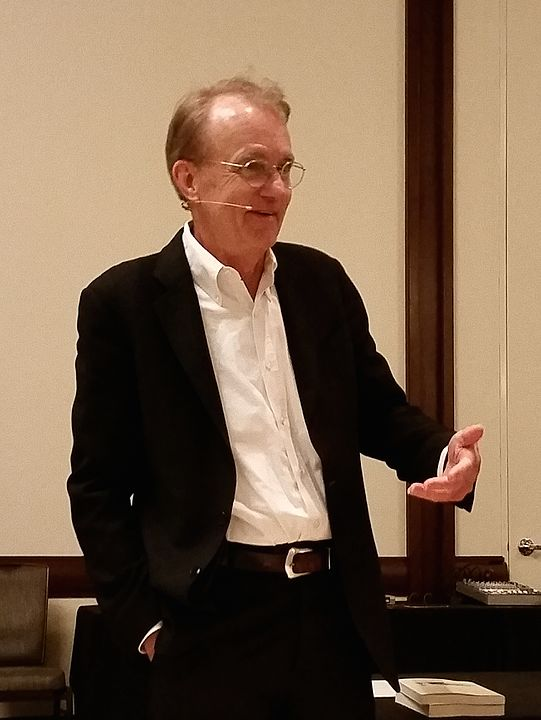
\includegraphics[width=0.25\textwidth,height=\textheight]{images/EdwardTufte.jpg}
(Source: Keegan Peterzell, CC BY-SA 4.0 \url{https://creativecommons.org/licenses/by-sa/4.0}, via Wikimedia Commons)

For Tufte, number one thing to learn about data visualization is to discard the default.

``If you're not doing something different, you're not doing anything at all.''
- Edward Tufte

\textbf{Example: Multiple dimensions of data}

\hypertarget{know-your-data}{%
\section{Know your data}\label{know-your-data}}

\begin{enumerate}
\def\labelenumi{\arabic{enumi}.}
\tightlist
\item
  Data Literacy
\item
  Data types
\item
  Visual Vocabulary
\end{enumerate}

\hypertarget{data-literacy}{%
\subsection{Data Literacy}\label{data-literacy}}

This course focuses on hands-on applications using real world data. It is advised students bring own dataset for practices. Sample programs will demonstrate how to import the data into R using base or add-on packages (e.g.~foreign, haven, vroom).

\hypertarget{hands-on-workshop-data-programming}{%
\subsection{Hands-on workshop: Data programming}\label{hands-on-workshop-data-programming}}

\hypertarget{data-programming}{%
\subsubsection{Data Programming}\label{data-programming}}

This session starts with basic principles for data programming or coding involving data. Data programming is a practice that works and evolves with data. Data programming or coding allows the user to manage and process data in more effective manner. Programs are designed to be replicated or replicable by user and collaborators. A data program can be developed and updated iteratively and incrementally. In other words, it is building on the culminated works without repeating the steps. It takes debugging, which is the process of identifying problems (bugs) but, in fact, updating the program in different situations or with different inputs when used in different contexts, including the programmer himself or herself working in future times.

\hypertarget{getting-started-with-rstudio-cloud}{%
\subsubsection{Getting started with RStudio Cloud}\label{getting-started-with-rstudio-cloud}}

RStudio is the most popular IDE for programming in R. It is very powerful and versatile, providing an environment for data science functions including managing, modeling and visualizing data. Above all those, RStudio is also equipped with tools to interface with other languages such as Python, Stan and SQL and creating a variety of output products such as LaTeX documents for press-ready publication and web-ready html files for web publication. This document is also prepared and rendered inside RStudio.

RStudio Cloud allows processing R programs in cloud using a browser only. This will free users from using local installation, which could sometimes be subject to hardware and/or operating system limits.

Steps to start RStudio Cloud:

\begin{enumerate}
\def\labelenumi{\arabic{enumi}.}
\tightlist
\item
  Use Google or GitHub account to login to the \href{http://Rstudio.cloud}{RStudio Cloud website}
\item
  At left menu, click on Your Workspace under Spaces.\\
\item
  Start a New Project (blue button on right) Project. Be sure to name your new project. A new R session will open.
\item
  You are ready to code and visualize data!
\end{enumerate}

\hypertarget{data-programming-in-r}{%
\subsubsection{Data programming in R}\label{data-programming-in-r}}

\emph{R basics}

\begin{Shaded}
\begin{Highlighting}[]
\CommentTok{# Create variables composed of random numbers using the rnorm function}
\NormalTok{x <-}\KeywordTok{rnorm}\NormalTok{(}\DecValTok{50}\NormalTok{) }
\NormalTok{y =}\StringTok{ }\KeywordTok{rnorm}\NormalTok{(x)}

\CommentTok{# Plot the points in the plane }
\KeywordTok{plot}\NormalTok{(x, y)}
\end{Highlighting}
\end{Shaded}

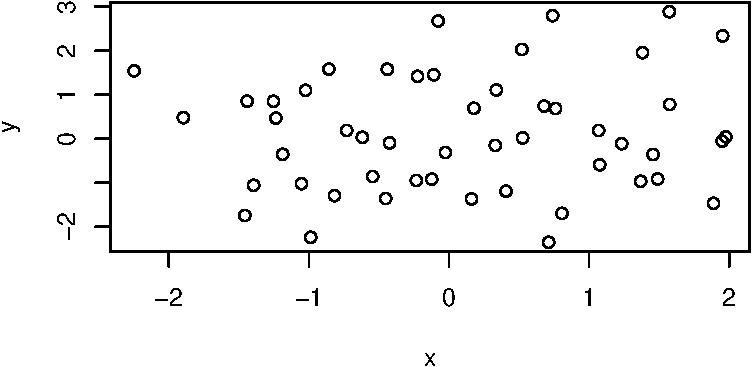
\includegraphics{book_dvp_files/figure-latex/unnamed-chunk-1-1.pdf}

\hypertarget{using-r-packages}{%
\subsubsection{Using R packages}\label{using-r-packages}}

\begin{Shaded}
\begin{Highlighting}[]
\CommentTok{# Plot better, using the ggplot2 package }
\CommentTok{## Prerequisite: install and load the ggplot2 package}
\CommentTok{## install.packages("ggplot2")}
\KeywordTok{library}\NormalTok{(ggplot2)}
\KeywordTok{qplot}\NormalTok{(x,y)}
\end{Highlighting}
\end{Shaded}

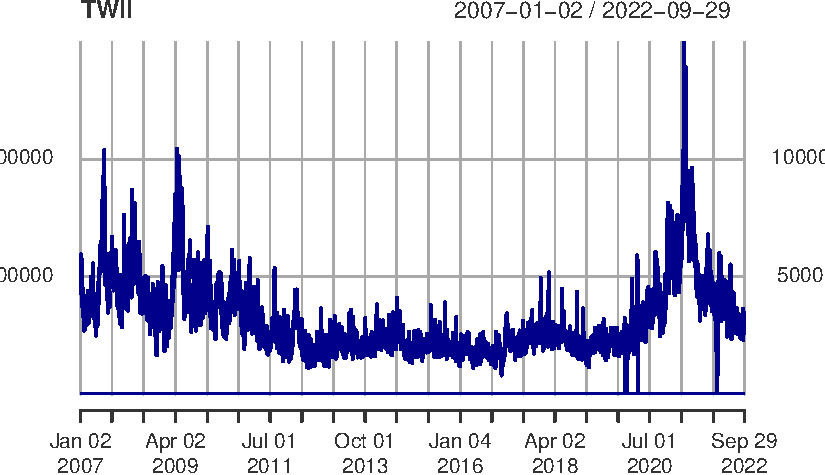
\includegraphics{book_dvp_files/figure-latex/unnamed-chunk-2-1.pdf}

\hypertarget{ggplot2-starter}{%
\subsection{ggplot2 starter}\label{ggplot2-starter}}

\begin{Shaded}
\begin{Highlighting}[]
\CommentTok{# Plot better better with ggplot2}
\NormalTok{x <-}\StringTok{ }\KeywordTok{rnorm}\NormalTok{(}\DecValTok{50}\NormalTok{) }
\NormalTok{y =}\StringTok{ }\KeywordTok{rnorm}\NormalTok{(x)}
\KeywordTok{ggplot}\NormalTok{(,}\KeywordTok{aes}\NormalTok{(x,y)) }\OperatorTok{+}\StringTok{ }\KeywordTok{theme_bw}\NormalTok{() }\OperatorTok{+}\StringTok{ }\KeywordTok{geom_point}\NormalTok{(}\DataTypeTok{col=}\StringTok{"blue"}\NormalTok{)}
\end{Highlighting}
\end{Shaded}

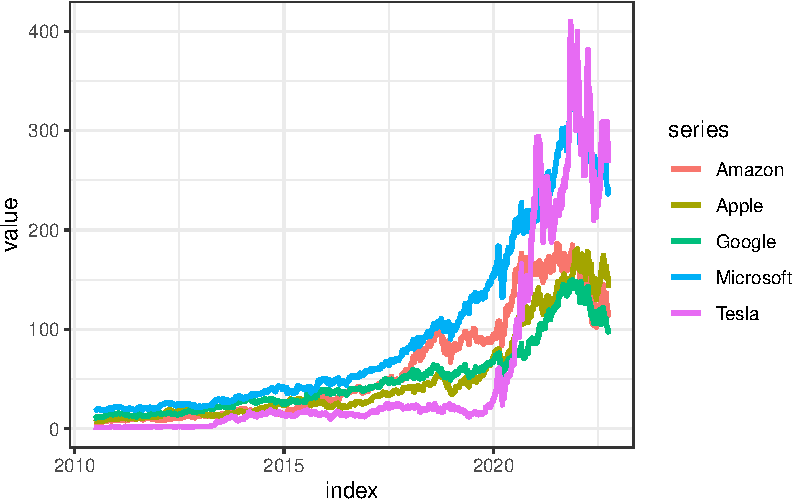
\includegraphics{book_dvp_files/figure-latex/unnamed-chunk-3-1.pdf}

\hypertarget{recommended-r-resources}{%
\subsubsection{Recommended R Resources:}\label{recommended-r-resources}}

\begin{itemize}
\tightlist
\item
  \href{http://journal.r-project.org/}{The R Journal}
\item
  \href{http://cran.r-project.org/doc/manuals/R-intro.pdf}{Introduction to R by W. N. Venables, D. M. Smith and the R Core Team}
\item
  \href{http://www.ats.ucla.edu/stat/r/seminars/intro.htm}{Introduction to R Seminar at UCLA}
\item
  \href{https://dss.princeton.edu/training/}{Getting Started in Data Analysis using Stata and R by Data and Statistical Services, Princeton University}
\end{itemize}

\hypertarget{references}{%
\subsubsection{References:}\label{references}}

Graham Williams 2011. \emph{Data Mining with Rattle and R: The Art of Excavating Data for Knowledge}

\hypertarget{functional}{%
\chapter{Functional approach}\label{functional}}

In this module, we will emphasize on hands-on applications, including building visual vocabulary, deciding chart types by function and data types and building charts using sample programs.

\hypertarget{interactive}{%
\chapter{Interactive}\label{interactive}}

We describe building interactive and reactive data visualization for web publication.

\hypertarget{ggiraph-package}{%
\section{ggiraph package}\label{ggiraph-package}}

\hypertarget{dash}{%
\section{Dash}\label{dash}}

\hypertarget{summary}{%
\chapter{Summary}\label{summary}}

In this brief three-day course, we have covered:

\begin{itemize}
\tightlist
\item
  Basics of data visualization
\item
  Building charts by functions (and data types)
\item
  Generating interactive data products
\end{itemize}

  \bibliography{book.bib,packages.bib}

\end{document}
